\documentclass[11pt,a4paper]{report}
\usepackage[utf8x]{inputenc}
\usepackage[french]{babel}
\usepackage[T1]{fontenc}
\usepackage{amsmath}
\usepackage{amsfonts}
\usepackage{amssymb}
\usepackage{graphicx}
\usepackage{listings}
\usepackage[left=2cm,right=2cm,top=2cm,bottom=2cm]{geometry}
\usepackage{natbib}


\usepackage[x11names]{xcolor}
\usepackage{booktabs}


\usepackage[%
 pdfstartview=FitH,%
 bookmarks=true,%
 bookmarksopen=true,%
 breaklinks=true,%
 colorlinks=true,%
 linkcolor=blue,anchorcolor=blue,%
 citecolor=blue,filecolor=blue,%
 menucolor=blue,%
 urlcolor=blue]{hyperref}

\lstdefinestyle{mystyle}{
breakatwhitespace=false,
    commentstyle=\color{gray},
    keywordstyle=\color{Green4},
    numberstyle=\footnotesize\color{gray},
    stringstyle=\color{purple},
    identifierstyle=\color{SteelBlue4},
    basicstyle=\ttfamily\small,
    numbers=left,
    keepspaces=false,
    numbers=left,
    showspaces=false,
    showstringspaces=true,
    }
\lstset{style=mystyle}

% \begin{lstlisting}[language=python]
% \end{lstlisting}

\begin{document}
\title{OpenPattern}
\author{F. Métivier}
\date{\today}
\maketitle

\tableofcontents


\chapter{Introduction}

\section{What is it}
OpenPattern  est une librairie python, orientée objet,  dont l'objectif est de permettre le tracé de patrons, en particulier de vêtements, à l'échelle 1:1 et leur sauvegarde au format pdf ou svg. Les patrons ainsi construits peuvent soit être directement imprimés pour utilisation soit être repris dans un logiciel de dessin comme Inkscape ou Illustrator.
OpenPattern offre la possibilité de créer des patrons «from scratch», d'utiliser des librairies de patrons existants (patrons de bases notamment) et de les reprendre pour les adapter et les transformer.

Les patrons peuvent être construits sur-mesures à partir d'un ensemble de mesures effectuées sur les corps d'une personne particulière (j'ai créé OpenPattern pour dessiner des vêtements pour ma famille), ou construits à partir de mesures de prêt à porter classique.

Les sources que j'ai utilisées pour tracer les patrons proviennent d'ouvrage de patronnages classiques. Ces ouvrages, destinés au couturiers amateurs ou aux étudiants d'écoles de modes, décrivent les techniques de réalisation de ce que l'on nomme la coupe à plat c'est-à-dire  la manière de projeter et tracer sur un plan (le papier puis le tissus) une forme géométrique 3D (le vêtement fini).

J'ai utilisé les ouvrages de quatre auteurs ou autrices principaux.
En premier lieu j'ai utilisé les quatre tomes de la série \textit{Le modélisme de mode} de Teresa Gilewska pour la femme et pour l'homme\cite{Gilewska1,Gilewska2,Gilewska4,Gilewska5}. J'ai aussi eu recours à deux tomes des ouvrages d'Antonnio Donnanno pour femme et homme également \cite{Donnanno2005,Donnanno2016}. Pour les enfants j'ai utilisé le tome correspondant de Jacqueline Chiapetta  \cite{Chiappetta1999} (mon préféré). Enfin pour l'homme j'ai aussi eu recours au livre de  Claire Wargnier sur le vestiaire masculin \cite{wargnier2012}. Ces ouvrages sont tous rédigés de façon similaire. Ils exposent, en procédant pas à pas, les techniques empiriques de tracé d'un body, d'un pantalon, d'une chemise etc.

la création d'un patron est donc une suite d'instruction comme «tracer un segment AB de longueur égale au 1/4 du tour de bassin» ou encore «ajouter une pince de 1.5 cm de 9cm de profondeur entre les points F1 et H» etc...
OpenPattern reprend de façon quasi litérale ces techniques et leur principe de construction en les adaptant quand cela se révèle nécessaire\footnote{Ces ouvrages présentent parfois des coquilles ou des imprécisions qui  sont probablement corrigées par leurs auteurs quand elles ou ils enseignent.}.


\section{How is it organized}

OpenPattern est organisée autour de classes qui héritent les unes des autres. Cette structure présente l'avantage de coller aux techniques de coupe. En effet une chemise, une veste ou un gilet sont des adaptations d'un body, une robe dérive de l'assemblage d'une jupe et d'un body, enfin les jupes et les pantalons dérivent de formes génériques dites de bases (jupe de base, pantalon de base).

OpenPattern présente pour l'instant deux niveaux d'héritage.
\begin{itemize}
\item La classe parente Pattern : C'est la classe générale qui définit ce qu'est un patron et les méthodes permettant de le dessiner et de le manipuler
\item Les classes de bases dérivées de Pattern: Basic\_Bodice, Basic\_Trousers, Cuffs, Collars
\item Les classes dérivées des classes de base: shirt, pyjamas qui héritent de Basic\_Bodice ou de Basic\_Trousers. \item Enfin les patrons font appels à une classe Point qui permet de définir un point de patronnage avec sa position et ses propriétés. Cette classe redéfinit les opérations d'addition et offre diverses manipulations  comme la rotation. L'intérêt ici est d'avoir un objet flexible qui permette de partir d'un patron de base et de l'altérer.
\end{itemize}

Pour dessiner un patron il faut
\begin{enumerate}
\item créer une instance de la classe correspondante,
\item appeler différentes méthodes d'altération ou de modification,
\item dessiner et, au besoin, sauvegarder le patron.
\end{enumerate}

Le dessin du patron peut aussi  directement se faire à partir des classes Pattern et Point comme nous allons le voir dans le tuto suivant.

\chapter{Tuto}


\section{Dessine moi un carré}

Le script suivant montre comment dessiner un carré (de tissus :=)).
les opérations consistent en
\begin{enumerate}
  \item la création du patron par la création d'une instance de la classe pattern,
  \item la création de quatre points,
  \item l'ajout de ces points au patrons,
  \item la définition de l'ordre dans lequel les tracés doivent être faits,
  \item enfin la représentation graphique.
\end{enumerate}

\lstinputlisting[language=Python]{./sample/simple_scripts_0.py}

la figure \ref{fig:carre} montre le résultat. Le patron du carré est constitué d'un carré grisé délimité par quatres segments dont les quatre sommets sont marqués par un point rouge avec son nom.  Le carroyage, qui donnent l'échelle et permet les raccords, fait 1 cm quand on imprime le patron en taille réelle. Le patron est enfin entouré d'une bande de 5cm de tous les côtés. Vous noterez qu'une échelle apparaît dans cette bande. Elle est automatiquement ajoutée avec l'option \texttt{save = True} c'est à dire quand votre patron finit mérite impression. Cela vous permettra de vérifier rapidement que votre patron est bien à l'échelle\footnote{Normalement les carrés font 1cm de côté mais une requête d'un ami m'a fait ajouter cette échelle (pour être certain que tout va bien dirons nous).}.

\begin{figure}
\begin{center}
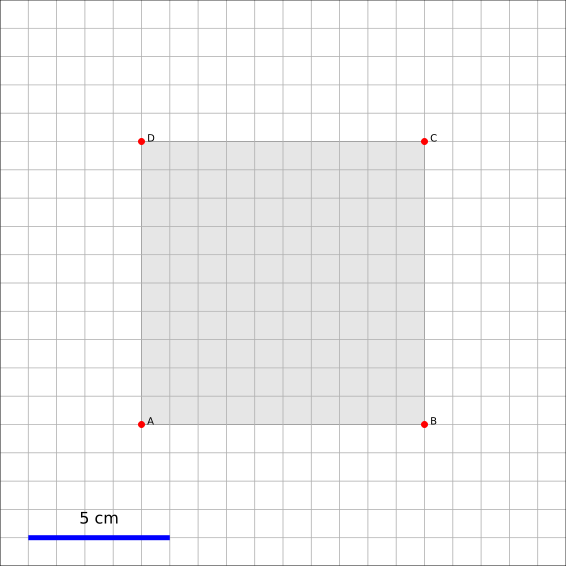
\includegraphics[width=0.6\textwidth]{../patterns/simple_scripts_0__FullSize}
\end{center}
\caption{Mon beau carré}
\label{fig:carre}
\end{figure}


\section{Dessine moi une pince}

Imaginons que nous allons transformer notre carré un peu pour en faire un demi-trapèze et lui ajouter une pince (Attention ça va faire jupe !). Les étapes sont les mêmes l'ajout de la pince se faisant évidemment après la définition des points du segment impacté par cet ajout.

\lstinputlisting[language=Python]{./sample/simple_scripts_1.py}

\begin{figure}
\begin{center}
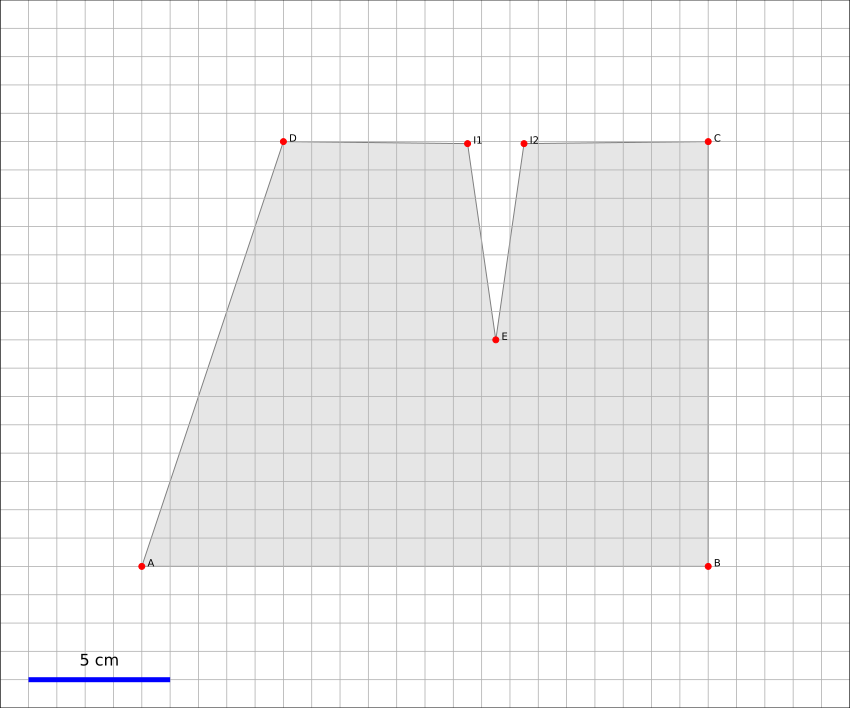
\includegraphics[width=0.6\textwidth]{../patterns/simple_scripts_1__FullSize}
\end{center}
\caption{Mon beau trapèze}
\label{fig:trapeze}
\end{figure}

Comme on le voit ici la création de la pince se fait en deux étapes. On définit la position du sommet de la pince puis on appelle la fonction \texttt{add\_dart} en lui passant quatre arguments (il y en a plus que nous verrons plus tard) le sommet, les deux points définissant le segment qui doit être pincé et la largeur de la pince. la fonction renvoie la position des deux points qui, avec le sommet, constitueront la pince sur le patron.  Il ne reste alors plus qu'à intercaler les points de pince lors de la définition du trajet du tracé. La figure \ref{fig:trapeze} montre le résultat. Comment ça elle ne vous plait pas ma jupe...

\section{Les légendes, marques et commentaires}

Un patron vient souvent accompagné de commentaires et de signes particulier comme l'indication du droit fil, les pliures et les crans de montages. Il est possible de les insérer sur votre patron à l'aide des commandes correspondantes comme le montre le script suivant et la figure qui l'accompagne (les commandes sont insérées dans le script précédent avant la commande \texttt{draw}).

\begin{lstlisting}[language=Python]
# add legends
myPattern.set_grainline(OP.Point([8,10]), 8, -np.pi/2)
myPattern.set_fold_line(C-[0,2], B+[0,2],'right')
myPattern.add_comment(OP.Point([12.5,15.5]),'TOP',0)
myPattern.add_comment(OP.Point([10,-0.5,]),'BOTTOM',0)


a = 70
myPattern.add_comment(OP.Point([2.8,8,]),'VV',a*np.pi/180) # workaround for notches
\end{lstlisting}


\begin{figure}
\begin{center}
\includegraphics[width=0.6\textwidth]{../patterns/simple_scripts_2__FullSize}
\end{center}
\caption{Mon beau trapèze et ses annotations}
\label{fig:trapeze}
\end{figure}

On notera au passage qu'à l'heure actuelle un cran de montage se place comme un commentaire constitué de V en série.

\section{Les courbes et le pistolet}

\section{Les annotations}

\section{Utiliser des mensurations}

\section{créer des patrons multiples}
Il est fréquent de créer un patron à partir de plusieurs bases différentes, buste et pantalon pour les salopettes par, buste et jupe pour certaines robes, ou encore buste, manche, col et manchette pour une chemise\footnote{On verra cependant dans ce dernier cas que la manche est intrinsèquement liée au buste. Elle vient «après» le dessin du buste}.

la classe \texttt{pattern} peut contenir d'autres \texttt{pattern} qui sont enregistrées dans la liste de patrons \texttt{pattern\_list}. Nous allons reprendre notre patron de jupe et le copier trois fois en utilisant des propriétés de translation et de rotation et de copie de la classe \texttt{pattern}.

\lstinputlisting[language=Python]{./sample/simple_scripts_3.py}


\begin{figure}
\begin{center}
\includegraphics[width=0.6\textwidth]{../patterns/simple_scripts_3__FullSize}
\end{center}
\caption{Patron composite: mon beau trapèze et ses trois avatars}
\label{fig:trapeze}
\end{figure}

La partie qui nous intéresse ici débute à la ligne 47. Il s'agit de copier le patron de départ dans P2, P3 et P4 puis de le translater ou lui faire faire une rotation par rapport à un de ses points. Enfin le patron est ajouter à la liste de sous-patrons de myPattern. Pour le dessin on commence par dessiner les sous patrons sur une même figure puis on dessine le patron principal et on ajoute les légendes. Enfin lors du dessin de sous-patrons vous pouvez activer l'overlay qui les dessine avec un remplissage plus léger dans le but de pouvoir dessiner les altérations par dessus ultérieurement dans la teinte de gris classique.





\section{Utiliser une classe dérivée}

Le script suivant montre par exemple comment tracer et sauver un patron de Body de femme sans pinces en 36 selon la méthode de Gilewska.
\begin{lstlisting}[language=python]
import sys
sys.path.append('./..')
import matplotlib.pyplot as plt
import OpenPattern as OP

p = OP.Basic_Bodice(pname = "W36G", gender = 'w', style = 'Gilewska') # Creation de l'instance
p.draw_bodice({"Pattern":"Bodice without dart"}, save=True) # appel de la fonction de dessin
plt.show() # si vous voulez voir la figure s'afficher
\end{lstlisting}

\begin{figure}[hbtp]
\centering
\includegraphics[width=0.7\linewidth]{../patterns/Gilewska_Bodice_withour_dart_36.pdf}
\caption{Gilweska style Women bodice with no dart. (size 36)}
\label{fig:bodice_WG36}
\end{figure}

On obtient alors la figure~\ref{fig:bodice_WG36} enregistrée par defaut à l'échelle 1:1 dans un fichier pdf.


Les différentes options sont passées dans les arguments des différentes méthodes de classe (draw\_bodice) ou lors des instanciations de classe (Basic\_Bodice dans cet exemple).

\begin{lstlisting}[language=python]
Basic_Bodice(pname="M44G", gender='m', style='Gilewska', age=12, ease=8, hip=True):
	"""
	Initilizes parent class &  attributes
	launches the calculation of bodice and sleeve
	saves measurements performed like armscye depth in the json measurements file for further processing in other classes

	Args:
		pname: size measurements
		gender: ..
		style: style to be used for drafting at present Gilewska, Donnanno and Chiapetta (for kids)
		age: used if for a child and style = Chiappetta.
		ease: ease in cm; used in Donnanno patterns
		hip: True/False use to decide for men whether to draw a fullbodice
	"""

draw_bodice(self, dic = {"Pattern":"Dartless bodice"}, save = False, fname = None, paper='FullSize'):
	""" Draws Basic Bodice with legends and save it if asked for

	Args:
		dic: dictionnary of informations to be printed
		save: if true save to file
		fname: filename
		paper: paper size on which to save (for cuts)
	"""
\end{lstlisting}

les figures~\ref{fig:bodice_DW36}, \ref{fig:bodice_MG36} et \ref{fig:CB14} montrent quelques exemples de body obtenus pour différents styles


\begin{figure}[hbtp]
\centering
\includegraphics[width=0.7\linewidth]{../patterns/Donnanno_Bodice_withour_dart_36.pdf}
\caption{Donnanno style Women bodice with no dart. (size 36)}
\label{fig:bodice_DW36}
\end{figure}

\begin{figure}[hbtp]
\centering
\includegraphics[width=0.7\linewidth]{../patterns/Gilewska_Bodice_withour_dart_M36.pdf}
\caption{Gilweska style Men bodice with no dart. (size 36)}
\label{fig:bodice_MG36}
\end{figure}

\begin{figure}[hbtp]
\centering
\includegraphics[width=0.7\linewidth]{../patterns/Chiappetta_bodice_G14.pdf}
\caption{Chiappetta style Boy (14 years old) bodice with no dart.}
\label{fig:CB14}
\end{figure}




\chapter{Les classes}

\section{Classe Pattern}
La liste des méthodes de cette classe est donnée ci-dessous. Ces méthodes sont à ce jour de trois types.

\begin{enumerate}
\item Les méthodes liées aux mesures qui permettent de charger ou d'enregistrer les modifications des mesures. Le choix pour l'instant est fait d'enregistrer les mesures dans des fichiers json.
\item Les méthodes de calculs couramment effectués en patronnage, mesurer une distance, un angle, chercher le point milieu d'un segment ou encore tracer une courbe. Ici le choix est fait d'utiliser des b-spline pour approximer le sacro-saint pistolet (on reviendra sur ce choix guidé au départ par la simplicité).
\item Les méthodes de dessin avec matplotlib.
\end{enumerate}

\subsection{Mesures}
Les mesures sont enregistrées dans une base de données sqlite3. Elles peuvent être enregistrées dans des fichiers json dans le répertoire measurements.

\begin{itemize}

\item Différences H/F
\subitem tour de poitrine vs tour de bassin: > chez les hommes, < chez les femmes
\subitem hauteur taille dos, taille devant: > chez les hommes, < chez les femmes

\item Intéressant de noter qu'en fait l'enfant garçon passe de l'un à l'autre à la puberté (cf Chiapetta)

\item Est-ce que ces différences sont à l'origine des différences de dessin ? probablement mais rien n'est expliqué (ou j'ai mal lu).
\end{itemize}


\section{Bodice}

\subsection{Naming convention}

trying to get standard
\begin{itemize}
\item		first letter Caps [then minor]
\begin{itemize}
\item		W: waist
\item		Sl: sleeve
\item		B: bust
\item		H: height
\item		C: collar
\item		Sh: shoulder
\item		DSl: depth of sleeve
\item		Cp: Control Point
\item		Hi: Hip
\end{itemize}

\item		Last Letter
\begin{itemize}
\item		B: Back
\item		F: Front
\end{itemize}

\item		No numbering when on the fold line numbering when on the sleeve side
\end{itemize}


Not done for Donnanno yet

\chapter{Commentaires}

Une fois n'est pas coutume, marché aidant probablement, les femmes sont mieux traitées que les enfants qui sont mieux traités que les hommes.

\section{Mesures}
ça part dans tous les sens notamment pour les hommes... le plus gros écart sépare ceux qui mesurent la largeur des épaules et ceux qui mesurent la longueur des épaules. Quelques un mesurent les deux mais c'est plus rare. On notera que les mesures type varient d'un livre à l'autre. Pas toujours de mesure du tour de bras, du tour de jaret, du tour de cuisse.

\section{Shoulder line}

Pour les femmes de style G, la  onstruction des épaules repose sur des angles fixes. Pour les hommes de style G, cela dépend des distances par rapport à la ligne des épaules comme podonc ur le style D. Pourquoi ce changement? Cela pose un problème car, si l'on suit les instructions, l'épaule est plus longue que les mesures (si elles existent) et les épaules avant et arrière n'ont pas la même longueur. Dans le cas où la longueur d'épaule est donnée, la solution est alors d'ajuster la longueur d'épaule à la longueur mesurée à laquelle la ligne d'épaule a été établie (comme suggéré par Donnanno). J'ai donc ajouté un test pour l'existence d'une mesure de la vraie longueur des épaules Si tel est le cas, la longueur de l'épaule est ajustée pour s'adapter aux mesures. Notons en outre que les largeurs d'épaules correspondent chez G homme si on ne baisse pas l'épaule devant de 7cm mais de 5 (comme chez Donnanno).


Pour les adolescents (garçons) de style C, l'épaule repose sur deux angles différents pour le dos (22 $ ^ o $) et le devant (25 $ ^ o $).



\section{Armhole and collar}

à noter que, encore une fois, pour l'homme tout est un peu fait par dessus
la jambe. Ok des chemises des pantalons et des costumes c'est pas
folichon mais quand même !

Donnano:  pour les femmes le buste de base présente un problème d'ajustement car il ne
fournit pas de points de contrôles. J'ai repris ceux de Gilweska.

Pour l'hommes: pas de buste de base j'en au  créé un à partir de la chemise de base.
relativement simple à faire. Par contre problème (toujours) pour les
longueurs d'épaule. La largeur d'épaule est donnée mais pas la
longueur (qui d'ailleurs n'est que très rarement donnée pour les
hommes). or on demande la longueur d'épaule (j'adore le e.g. 17cm mis
dans l'exemple dont on ne sait pas d'où il sort)

Gilewska : pour le buste homme j'ai ajouté  deux points de contrôle
en base de manche  afin d'assurer la platitude d'emmanchure. Sinon les
spleen ne veulent pas faire comme le perroquet.


Chiappetta pour adolescents: (figure ~ \ ref {fig: CB14}) n'utilise qu'une seule mesure de carrure celle du dos. Pour les adolescents de plus de 10 ans, elle récupère juste deux cm de carrure mesurés au dos pour le devant. Le collier arrière a besoin d'un deuxième point de contrôle près de la ligne de pliage pour assurer la planéité de la cannelure.

Pour l'enfant Chiapetta changer l'angle, la longueur des points de contrôle et la carrure devant. de 2 à 8 ans les angles d'épaule devant et derrière sont les même, les longueurs plus petites et la carrure devant et dos sont les mêmes.

L'emmanchure et l'encolure sont faites avec des splines de second ordre. J'ai fini par jouer sur le fit des splines et les points de contrôle. À développer.

Bon mais comme d'hab Chiapetta ça à l'air un peu ringard sur les bords mais ça marche tout seul. je pense que je vais investir dans
les bouquins adultes notamment pour l'homme...


\section{Manches}
Gilewska: Aucune indication pour le bas de manche de base il faut donc
se débrouiller seul avec le tour de poignet...

Les splines ici sont du troisième ordre car il y a un point d'inflexion.


De façon générale je trouve que les bustes hommes ne sont pas très ressemblant aux dessins des livres et je suis dubitatif car le programme reproduit exactement les instruction sauf quand c'est problématique de façon évidente (genre les largeur d'épaules de Donnanno).


\section{Collars}
Styles available from Gilewska men: Officer and OnePiece (for one piece collar)

\begin{figure}
\begin{center}
\includegraphics[width=0.48\textwidth]{../patterns/collar_Gilewska_OnePiece_M44G_FullSize.pdf}
\includegraphics[width=0.48\textwidth]{../patterns/collar_Gilewska_Officer_M44G_FullSize.pdf}
\end{center}
\caption{Collar styles}
\end{figure}


\section{Cuffs}
Styles availabel from Gilewska men : Simple and French

\begin{figure}
\begin{center}
\includegraphics[width=0.48\textwidth]{../patterns/cuff_Gilewska_Simple_M44G_FullSize.pdf}
\includegraphics[width=0.48\textwidth]{../patterns/cuff_Gilewska_French_M44G_FullSize.pdf}
\end{center}
\caption{Cuff styles}
\end{figure}

\section{Trousers}


\subsection{Pants Block}

Incohérence du modèle chez Donnanno. La mesure de la ceinture est
$$AV = Hip + 6.$$
Or la somme
$$ceinture avant + ceinture arriere = Hip +2.$$
Donanno indique qu'il faut séparer les patrons avant et arrière de 6cm soit
$$ceinture avant + ceinture arriere + 6 = Hip +8 = AV,$$
d'où l'incohérence.


\bibliographystyle{plain}
\bibliography{OpenPattern.bib}

\end{document}
